% =====================================================================
\chapter{Conductors and Capacitance}

A conductor is a material containing charges that are free to move in response to any electric field present. That single property, combined with the demand that nothing be moving, is enough to fix a great deal: the field inside, the charge density inside, the direction and magnitude of the field at the surface, and the behaviour of the potential throughout. This chapter derives each of those in turn, then uses them to develop capacitance, first for a single pair of conductors and then for an arbitrary system of them.

% =====================================================================
\section{Electrostatic Equilibrium}
% =====================================================================

Throughout we consider a conductor in \emph{electrostatic equilibrium}: nothing is moving, and all quantities are time-independent. Everything in this section is a consequence of that assumption alone, holding regardless of the conductor's shape or of what other charges are present nearby.

\begin{theorem}[The interior field vanishes]
$\vect{E} = 0$ at every point in the interior of a conductor in electrostatic equilibrium.
\end{theorem}

\begin{proof}
Suppose, for contradiction, that $\vect{E}\neq 0$ at some interior point. The free charges there feel a force $\vect{F} = q\vect{E}\neq 0$, and by Newton's second law they accelerate. But moving charges contradict the assumption that the configuration is static. Hence no such point can exist, and $\vect{E} = 0$ throughout the interior.
\end{proof}

This is a statement about the \emph{full} vector, not merely its magnitude or one of its components --- a point we will need shortly. Note also what it does not say: the field outside is not zero, and the conductor does not shield its exterior. What has happened physically is that the free charges redistribute themselves until the field they produce exactly cancels whatever external field is applied. An insulator has no such freedom, and the external field penetrates it essentially unchanged.

\begin{figure}[H]
\begin{center}
\begin{tikzpicture}[scale=0.9]
  % External field arrows (left side: insulator)
  \foreach \y in {-1.2,-0.6,0,0.6,1.2} {
    \draw[-{Stealth[length=4pt]}, gray!60] (-4.0,\y) -- (-2.6,\y);
    \draw[-{Stealth[length=4pt]}, gray!60] (-1.4,\y) -- (-0.2,\y);
  }
  % Insulator body
  \fill[yellow!15] (-2.5,-1.4) rectangle (-1.5,1.4);
  \draw[thick] (-2.5,-1.4) rectangle (-1.5,1.4);
  \node[font=\small] at (-2.0,-1.7) {Insulator};
  \node[font=\small] at (-2.0,0) {$\vect{E}$ unchanged};

  % Conductor (right side)
  \fill[gray!20] (1.5,-1.4) rectangle (2.5,1.4);
  \draw[thick] (1.5,-1.4) rectangle (2.5,1.4);
  \node[font=\small] at (2.0,-1.7) {Conductor};
  % Induced charges
  \foreach \y in {-1.0,-0.5,0,0.5,1.0} {
    \node[red, font=\small] at (1.65,\y) {$-$};
    \node[blue!70!black, font=\small] at (2.35,\y) {$+$};
  }
  % Internal E = 0 label
  \node[font=\small, orange!80!black] at (2.0,0) {$\vect{E}=0$};
  % External field arrows
  \foreach \y in {-1.2,-0.6,0,0.6,1.2} {
    \draw[-{Stealth[length=4pt]}, gray!60] (0.2,\y) -- (1.4,\y);
    \draw[-{Stealth[length=4pt]}, gray!60] (2.6,\y) -- (3.8,\y);
  }
\end{tikzpicture}
\end{center}
\caption{Insulator vs.\ conductor in an external field. In the insulator there is no internal redistribution; in the conductor free charges migrate until the internal field cancels, giving $\vect{E}=0$ inside.}
\end{figure}

The vanishing of the interior field immediately constrains where charge can sit.

\begin{theorem}[Charge resides on the surface]
The volume charge density $\rho$ vanishes throughout the interior of a conductor, and any excess charge resides entirely on its surface.
\end{theorem}

\begin{proof}
Gauss's law in local form reads $\div\vect{E} = \rho/\varepsilon_0$. Since $\vect{E} = 0$ at every interior point, its divergence is identically zero there as well, forcing $\rho = 0$ throughout the interior. Any net charge placed on the conductor therefore cannot reside in the bulk; it must live as a surface charge density $\sigma$ on the boundary.
\end{proof}

In the idealized macroscopic treatment used here that surface charge is a genuine two-dimensional sheet. Microscopically the layer has a finite, atomic-scale thickness, but that refinement plays no role in anything below.

\begin{example}[Spherically Symmetric Field --- Neutral Conducting Spherical Shell]
Consider a neutral conducting spherical shell enclosing a point charge $q$. A Gaussian surface drawn inside the shell material encloses zero flux, so zero net charge; since the enclosed charge $q$ is already there, the inner surface must carry $-q$. The outer surface then carries $+q$ to keep the conductor neutral overall. The external field is purely radial, identical to that of a point charge $+q$ at the center --- even if $q$ is off-center inside.

\begin{figure}[H]
\begin{center}
\begin{tikzpicture}[scale=0.9]
  % Shell material (annulus)
  \fill[gray!25, even odd rule] (0,0) circle (2.4) (0,0) circle (1.6);
  \draw[thick] (0,0) circle (2.4);
  \draw[thick] (0,0) circle (1.6);
  % Point charge inside the cavity, deliberately off-centre
  \filldraw[red] (-0.55,0.35) circle (2.5pt);
  \node[red, font=\small, right] at (-0.42,0.38) {$q$};
  % Induced charge: -q on the inner surface, +q on the outer surface
  \foreach \a in {0,40,...,320} {\node[red, font=\small] at (\a:1.78) {$-$};}
  \foreach \a in {0,30,...,330} {\node[blue!70!black, font=\small] at (\a:2.24) {$+$};}
  % Gaussian surface drawn wholly inside the metal
  \draw[dashed, black!60] (0,0) circle (2.02);
  % External field: purely radial
  \foreach \a in {45,90,135,180,225,270,315} {
    \draw[-{Stealth[length=4pt]}, thick, orange!80!black] (\a:2.55) -- (\a:3.3);
  }
  % Labels
  \draw[->, gray] (3.6,2.3) -- (34:2.4);
  \node[font=\small, right] at (3.55,2.35) {outer surface: $+q$};
  \draw[->, gray] (3.6,-2.3) -- (-38:1.6);
  \node[font=\small, right] at (3.55,-2.35) {inner surface: $-q$};
  \draw[->, gray] (-3.9,-2.3) -- (-1.55,-1.35);
  \node[font=\small, left] at (-3.85,-2.35) {Gaussian surface};
  \draw[->, gray] (-3.9,1.9) -- (-2.02,1.0);
  \node[font=\small, left] at (-3.85,1.95) {metal: $\vect{E}=0$};
  \node[font=\small, orange!80!black] at (0,-3.95) {outside: $\vect{E}$ radial, as for $+q$ at the center};
\end{tikzpicture}
\end{center}
\caption{Point charge $q$ inside a neutral conducting shell: the inner surface carries $-q$, the outer surface $+q$, and the outside field is that of $+q$ at the center.}
\end{figure}
\end{example}

% =====================================================================
\section{The Field at the Surface}
% =====================================================================

We now determine $\vect{E}$ immediately outside the conductor's surface. The field there is a vector, so it must be pinned down twice: once for the component normal to the surface, and once for the component tangential to it. The two require different arguments and different constructions, and it is worth keeping them separate, since a common error is to suppose that the pillbox below settles both.

\subsection{The Normal Component: a Gaussian Pillbox}

\begin{figure}[H]
\begin{center}
\begin{tikzpicture}[scale=1.0]
  \fill[gray!20] (-3,-1.6) rectangle (3,0);
  \draw[thick] (-3,0) -- (3,0);
  \node[font=\small] at (0,-0.9) {conductor ($\vect{E}=0$)};
  \draw[dashed, black!70] (-0.6,-0.5) rectangle (0.6,0.6);
  \node[font=\small] at (0,-0.28) {$E=0$};
  \draw[-{Stealth[length=5pt]}, thick, orange!80!black] (0,0.6) -- (0,1.6)
    node[right, font=\small] {$\vect{E}=\tfrac{\sigma}{\varepsilon_0}\hat{n}$};
  \foreach \x in {-0.3,0,0.3} {\node[blue!70!black, font=\small] at (\x,0.12) {$+$};}
  \node[font=\small, black!60] at (1.55,0.25) {area $A$};
\end{tikzpicture}
\end{center}
\caption{A Gaussian pillbox straddling the surface. The inner face contributes no flux because $\vect{E}=0$ inside, and the side wall contributes none in the limit of vanishing height, so the entire flux $\sigma A/\varepsilon_0$ passes through the outer face.}
\end{figure}

Take a small pillbox --- a short cylinder --- straddling the surface, with one flat face of area $A$ just inside the conductor, the other just outside, and a connecting side wall of negligible height, so that its flux contribution vanishes. Gauss's law in integral form gives
\[
    \oint_S \vect{E}\cdot\hat{n}\,da = \frac{Q_\text{enc}}{\varepsilon_0}.
\]
The inside face contributes nothing, since $\vect{E} = 0$ there, and the enclosed charge is $Q_\text{enc} = \sigma A$. The entire flux therefore comes from the outside face alone:
\[
    E_\perp A = \frac{\sigma A}{\varepsilon_0} \quad\Longrightarrow\quad E_\perp = \frac{\sigma}{\varepsilon_0}.
\]
This fixes only the component of $\vect{E}$ normal to the surface. The pillbox says nothing whatever about any component lying \emph{within} the surface, since such a component would contribute no flux through either face.

\subsection{The Tangential Component: a Thin Rectangular Loop}

\begin{figure}[H]
\begin{center}
\begin{tikzpicture}[scale=1.0]
  \fill[gray!20] (-3.4,-2.2) rectangle (3.4,0);
  \draw[thick] (-3.4,0) -- (3.4,0);
  \node[font=\small] at (0,-1.5) {conductor};
  \draw[dashed, black!70] (-1.6,-0.8) rectangle (1.6,0.8);
  \draw[-{Stealth[length=5pt]}, thick, orange!80!black] (-1.3,0.45) -- (1.3,0.45);
  \node[font=\small, orange!80!black] at (0,1.15) {$E_{\parallel,\text{out}}$};
  \draw[-{Stealth[length=5pt]}, thick, black!55] (1.3,-0.45) -- (-1.3,-0.45);
  \node[font=\small, black!55] at (0,-1.0) {$E_{\parallel,\text{in}}=0$};
  \draw[<->, gray, thin] (1.95,-0.8) -- (1.95,0.8) node[midway, right, font=\small] {$h\to 0$};
  \draw[<->, gray, thin] (-1.6,1.75) -- (1.6,1.75) node[midway, above, font=\small] {$L$};
\end{tikzpicture}
\end{center}
\caption{A thin rectangular loop straddling the surface. As $h\to 0$ the short sides contribute nothing to the circulation, so the two long sides must cancel one another.}
\end{figure}

Take instead a thin rectangular loop straddling the surface: two long sides of length $L$ running parallel to the surface, one just outside and one just inside, joined by two short sides of length $h$, with $h\to 0$ at the end. The electrostatic field is curl-free, since it derives from a scalar potential, so
\[
    \oint \vect{E}\cdot d\vect{\ell} = 0
\]
around any closed loop. The short sides contribute at most $|\vect{E}|_{\max} h$, which vanishes as $h\to 0$, so only the two long sides survive. They are traversed in opposite directions in order to close the loop, whence the relative sign:
\[
    E_{\parallel,\text{out}}\,L - E_{\parallel,\text{in}}\,L = 0 \quad\Longrightarrow\quad E_{\parallel,\text{out}} = E_{\parallel,\text{in}}.
\]
Here is where it matters that the first theorem gave us the vanishing of the entire interior vector and not merely its normal part: $E_{\parallel,\text{in}} = 0$, and therefore $E_{\parallel,\text{out}} = 0$ as well.

\subsection{The Combined Result}

\begin{formula}[Field just outside a conductor]
\[
    \vect{E}_\text{just outside} = \frac{\sigma}{\varepsilon_0}\,\hat{n},
\]
directed straight out of the surface, with no component running along it. Equivalently, in terms of the potential, $\sigma = -\varepsilon_0\,\pdv*{\phi}{n}$, where $\pdv*{}{n}$ is the outward normal derivative.
\end{formula}

Field lines therefore always meet a conductor's surface at a right angle. The physical reading is a consistency check on the assumption we started from: were a tangential component to exist, free charges sitting at the surface would feel a force \emph{along} the surface and would begin to slide, contradicting equilibrium. The mathematics and the physics agree, as they must.

% =====================================================================
\section{The Conductor as an Equipotential}
% =====================================================================

\begin{theorem}[A conductor is an equipotential]
The scalar potential $\phi$ is constant throughout the interior of a conductor, and takes that same constant value on its entire surface.
\end{theorem}

\begin{proof}
Recall that for any path $\gamma$ running from a point $P$ to a point $Q$,
\[
    \phi(Q) - \phi(P) = -\int_\gamma \vect{E}\cdot d\vect{\ell}.
\]

\textbf{Step 1 (the interior).} Let $P$ and $Q$ be any two interior points. The interior is connected, so choose a path $\gamma$ from $P$ to $Q$ lying entirely within the conductor. Because $\vect{E} = 0$ at \emph{every} point of the interior, the integrand vanishes identically along the whole path --- no appeal to path independence or to Stokes's theorem is needed here, since the field being integrated is zero everywhere on the path, whatever its shape. Hence
\[
    \phi(Q) - \phi(P) = -\int_\gamma 0\,d\ell = 0 .
\]
Since $P$ and $Q$ were arbitrary, $\phi \equiv \phi_0$ for some constant $\phi_0$ throughout the interior.

\textbf{Step 2 (the surface).} Let $R$ be a point on the surface, and let $P_n\to R$ be a sequence of interior points approaching it, say along the inward normal. Each $P_n$ is interior, so $\phi(P_n) = \phi_0$ for every $n$ by Step 1. The potential is continuous across an ordinary charged surface --- a finite surface-charge sheet, as opposed to an idealized dipole layer, which does produce a jump --- so continuity gives
\[
    \phi(R) = \lim_{n\to\infty}\phi(P_n) = \phi_0 .
\]
As $R$ was an arbitrary surface point, $\phi = \phi_0$ on the entire surface as well.
\end{proof}

\begin{figure}[H]
\begin{center}
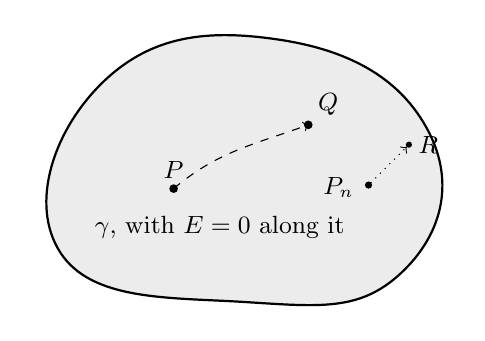
\begin{tikzpicture}[scale=0.9]
  \draw[fill=gray!15, thick] plot[smooth cycle, tension=0.8] coordinates {(-2.6,-1.1) (-2,1.3) (0.5,1.9) (2.6,0.6) (2.2,-1.4) (0,-1.8)};
  \filldraw (-1.0,-0.2) circle (1.5pt) node[above, font=\small] {$P$};
  \filldraw (0.9,0.7) circle (1.5pt) node[above right, font=\small] {$Q$};
  \draw[->, dashed] (-1.0,-0.2) to[out=40,in=200] (0.9,0.7);
  \node[font=\small] at (-0.35,-0.75) {$\gamma$, with $\vect{E}=0$ along it};
  \filldraw (1.75,-0.15) circle (1.2pt);
  \node[font=\small, left] at (1.68,-0.18) {$P_n$};
  \filldraw (2.32,0.42) circle (1pt) node[right, font=\small] {$R$};
  \draw[->, dotted] (1.78,-0.12) -- (2.29,0.39);
\end{tikzpicture}
\end{center}
\caption{Proving the conductor is an equipotential. Any interior path $\gamma$ has $\vect{E}=0$ along it, so all interior points share one potential; continuity of $\phi$ then carries that value out to each surface point $R$ as a limit of interior points $P_n$.}
\end{figure}

\subsection{Shielding: No Field Lines Within a Conductor}

An immediate corollary is that no field line can run through the material of a conductor. Such a line would join two distinct points $A$ and $B$ of the conductor with $\vect{E}\neq 0$ along it, giving $\phi(B)-\phi(A) = -\int_A^B\vect{E}\cdot d\vect{\ell} \neq 0$ and contradicting the constancy just proved. This is the basis of \textbf{electrical shielding}.

% =====================================================================
\section{Field Lines Between Conductors at Different Potentials}
% =====================================================================

Let conductors $A$ and $B$ be held at potentials $\phi_A > \phi_B$, and consider a field line leaving $A$ at a point $P$ and terminating on $B$ at a point $Q$; by the previous section it leaves and arrives perpendicular to both surfaces. Along this line,
\[
    \phi_B - \phi_A = \phi(Q) - \phi(P) = -\int_P^Q \vect{E}\cdot d\vect{\ell} < 0 .
\]
The left-hand side is negative by hypothesis. For the right-hand side to be negative as well, with $d\vect{\ell}$ oriented along the direction of travel from $P$ to $Q$, the integrand $\vect{E}\cdot d\vect{\ell}$ must be positive on average along the path --- that is, $\vect{E}$ must have a positive component along the direction running from $A$ to $B$.

\begin{fact}
Field lines point from the higher-potential conductor toward the lower-potential one.
\end{fact}

This matches the familiar statement that a positive test charge, feeling $\vect{F} = q\vect{E}$, is pushed from high potential to low. The point is that it is now a consequence of the line-integral relation rather than a separate assumption.

\begin{figure}[H]
\begin{center}
\begin{tikzpicture}[scale=0.85]
  \draw[fill=gray!15, thick] (0,0) ellipse (1.5cm and 1.1cm);
  \node at (0,0.15) {$A$};
  \node[font=\small] at (0,-0.35) {$\phi_A$};
  \draw[fill=gray!15, thick] (5.5,0) ellipse (1.5cm and 1.1cm);
  \node at (5.5,0.15) {$B$};
  \node[font=\small] at (5.5,-0.35) {$\phi_B$};
  \draw[-{Stealth[length=5pt]}, thick, orange!80!black] (1.45,0.55) to[out=20,in=160] (4.05,0.55);
  \draw[-{Stealth[length=5pt]}, thick, orange!80!black] (1.5,0) -- (4.0,0);
  \draw[-{Stealth[length=5pt]}, thick, orange!80!black] (1.45,-0.55) to[out=-20,in=200] (4.05,-0.55);
  \node[font=\small] at (2.75,-1.45) {$\phi_A>\phi_B \;\Rightarrow\; \vect{E}$ points $A\to B$};
\end{tikzpicture}
\end{center}
\caption{Field lines running between two conductors at different potentials. They leave both surfaces perpendicularly and are directed from the higher potential to the lower.}
\end{figure}

% =====================================================================
\section{Summary of Conductor Properties}
% =====================================================================

\begin{formula}[Conductor properties in electrostatic equilibrium]
For any conductor in equilibrium, whatever its shape and whatever external charges are present:
\begin{enumerate}
    \item $\vect{E} = 0$ everywhere in the material.
    \item $\rho = 0$ in the material; all net charge sits on the surface as $\sigma$.
    \item $\phi$ is constant over the material and its surface: $\phi_a = \phi_b$ for any two points of one conductor.
    \item Just outside, $\vect{E} = (\sigma/\varepsilon_0)\,\hat{n}$ --- perpendicular to the surface, with no tangential part --- so that $\sigma = -\varepsilon_0\,\pdv*{\phi}{n}$ and $Q_\text{enc} = \oint\sigma\,da = \varepsilon_0\oint\vect{E}\cdot d\vect{a}$.
    \item No field line passes through the material, which is what makes a conductor a shield.
\end{enumerate}
\end{formula}

% =====================================================================
\section{The Boundary-Value Problem and Uniqueness}
% =====================================================================

Because $\phi$ is a scalar it is easier to work with than $\vect{E}$. We seek $\phi$ satisfying $\laplacian\phi = 0$ --- or $-\rho/\varepsilon_0$ where charge is present --- subject to boundary conditions on the conducting surfaces that bound the region. Such a \textbf{boundary-value problem} is fully specified either by prescribing $\phi$ on each conductor, or equivalently by specifying the total charge $Q_k$ on each one.

\begin{theorem}[3.1 (Uniqueness Theorem)]
Assuming that there is a solution $\phi(x,y,z)$ for a given set of conductors with potentials $\phi_{0i}$, this solution must be unique.

\textbf{Proof idea:} Assume there is another solution $\psi(x,y,z)$. Since $\laplacian\phi = 0$ is linear, $\phi + c\psi$ is also a solution for $c_1\phi + c_2\psi$. In particular, let $W(x,y,z) \defeq \phi - \psi$. But then $W$ is not a solution because $\phi(\text{boundary}) = \psi(\text{boundary}) \neq 0$, but $W(\text{boundary}) = \phi(\text{boundary}) - \psi(\text{boundary}) = 0$. So $W$ is the solution to a different problem where the same conductors but all conductors held at 0 potential.

$\Rightarrow$ $W$ must be 0 everywhere (if not, then it violates the fact that it has a maximum $\phi^\text{avg}_\text{inner}$, since it has no maximum).

$\Rightarrow$ $\psi = \phi$ everywhere.

This theorem also works when there is charge: $\laplacian\phi = -\dfrac{\rho}{\epsilon_0}$.
\end{theorem}

This is powerful: if you can guess a solution --- by images, by symmetry, by any means at all --- that satisfies Laplace's equation and matches every boundary condition, then it must be \emph{the} solution. Every technique in the remainder of the chapter rests on that licence.

\begin{theorem}[Corollary 3.2]
In the space inside a hollow conductor of any shape, if that space is empty of charge, the electric field is 0.

\textbf{Proof:} Since $\phi$ is equipotential on the boundaries of the conductor, and thus by the \emph{average-value condition} must be $\phi_0$ throughout the entire region enclosed by the conductor. $\Rightarrow \vect{E} = 0$.

This is related to the proof that $\vect{E} = 0$ on the inside of a conductor; since neutral atom $=$ empty space.
\end{theorem}

% =====================================================================
\section{The Method of Images}
% =====================================================================

The method of images is uniqueness put to work. We replace a conductor by one or more fictitious \emph{image} charges chosen so that the boundary condition on the conductor's surface is reproduced exactly; the resulting field, in the physical region, is then guaranteed to be the right one.

Consider a point charge $+q$ at height $h$ above an infinite grounded conducting plane, so that $\phi = 0$ on the plane.

\begin{figure}[H]
\begin{center}
\begin{tikzpicture}[scale=0.95]
  % Conducting plane
  \fill[gray!25] (-3.0,-0.2) rectangle (3.0,0.0);
  \draw[thick] (-3.0,0) -- (3.0,0) node[right]{$\Phi=0$};
  % Real charge +q above
  \filldraw[red] (0,1.8) circle (4pt) node[right]{$+q$};
  % Height label
  \draw[<->, gray, thin] (0.4,0) -- (0.4,1.8) node[midway,right]{$h$};
  % Image charge -q below (dashed)
  \filldraw[blue!70!black] (0,-1.8) circle (4pt) node[right]{$-q$ (image)};
  \draw[dashed, blue!50!black] (0,-1.8) -- (0,0);
  % Field lines arching from +q to plane
  \foreach \x in {-1.2,-0.5,0.5,1.2} {
    \draw[thick, orange!80!black, -{Stealth[length=4pt]}]
      (0,1.8) .. controls (\x,1.0) and (\x,0.3) .. (\x,0);
  }
  % Note
  \node[font=\small, gray] at (-2.5,-1.0) {(image construction)};
\end{tikzpicture}
\end{center}
\caption{A point charge $+q$ at height $h$ above a grounded conducting plane ($\Phi=0$). Field lines meet the plane perpendicularly. The image charge $-q$ at $-h$ reproduces the same boundary conditions.}
\end{figure}

Place a mirror image charge $-q$ at depth $-h$ below the plane. On the plane every point is equidistant from the two charges, so their potentials cancel there and $\phi = 0$ over the whole plane; by symmetry the field is also perpendicular to it. Both boundary conditions are thus satisfied, and the two-charge system solves Laplace's equation everywhere above the plane, where no image charge is located. By uniqueness, the field in the physical region $z>0$ is exactly that of the two-charge system --- even though the image charge does not exist.

\subsection{The Induced Surface Charge}

With the field in hand we can compute what the conductor actually carries. At a distance $r$ from the foot of the charge, the two contributions have equal magnitude and their horizontal parts cancel, leaving a purely vertical field of magnitude $2\,|\vect{E}_q|\cos\theta$ with $\cos\theta = h/\sqrt{r^2+h^2}$:
\[
    E_z = -\frac{2q}{4\pi\varepsilon_0\,(r^2+h^2)}\cdot\frac{h}{\sqrt{r^2+h^2}} = -\frac{qh}{2\pi\varepsilon_0\,(r^2+h^2)^{3/2}} .
\]
Returning to the original problem, the boundary condition of the previous section gives $E_z = \sigma/\varepsilon_0$ just above the plane, whence
\[
    \sigma(r) = -\frac{qh}{2\pi\,(r^2+h^2)^{3/2}} .
\]
The induced charge is densest directly beneath the point charge and falls off as $r^{-3}$ far away. Integrating it over the plane, with the area element $2\pi r\,dr$,
\[
    Q_\text{induced} = \int_0^\infty \sigma(r)\,2\pi r\,dr
    = -qh\int_0^\infty \frac{r\,dr}{(r^2+h^2)^{3/2}}
    = -qh\left[\frac{-1}{\sqrt{r^2+h^2}}\right]_0^\infty = -q ,
\]
so the plane draws up exactly the charge of the image it is standing in for --- a satisfying check that the construction is doing what we asked of it.

\subsection{General Strategy}

Given the solution to any electrostatic problem, with its equipotential surfaces located, one obtains the solution to a new problem by ``copper-plating'' any one of those equipotentials: the field on either side is unchanged, because a conducting surface placed along an equipotential imposes exactly the boundary condition that surface already satisfied. Reading this backwards is the method of images --- replace the conductor by whatever charge configuration would have produced that equipotential in the first place.

% =====================================================================
\section{Capacitance}
% =====================================================================

An isolated conductor carrying charge $Q$ acquires a potential $\phi_0$, measured with respect to zero at infinity. By the linearity of Laplace's equation, doubling the charge doubles the potential everywhere, so $Q\propto\phi_0$ with a constant of proportionality that depends only on the geometry.

\begin{formula}[Capacitance (isolated conductor)]
\[
    Q = C\phi_0
\]
\[
    [C] = \frac{\text{Coulomb}}{\text{Volt}} = 1\,\text{Farad}
\]
($\epsilon_0$ can be expressed as Farads/metre.)
\end{formula}

For an isolated sphere of radius $a$, $\phi_0 = Q/4\pi\varepsilon_0 a$, so $C = 4\pi\varepsilon_0 a$. For an isolated conducting disk of the same radius, $C = 8\varepsilon_0 a$: a disk needs less charge than a sphere to reach a given potential.

\subsection{Two Conductors}

\begin{definition}[Capacitor]
A capacitor consists of two conductors with potentials $\phi_1$ and $\phi_2$, charges $+q$ and $-q$:
\[
  Q = C\bigl(|\phi_1 - \phi_2|\bigr) \quad \text{only valid if you move } Q
  \text{ from one previously neutral conductor}
\]
\[
  Q \approx C\Phi = C|\Delta\phi|
\]
\end{definition}

More usefully, for a pair of conductors carrying $+Q$ and $-Q$ the capacitance is referred to their potential \emph{difference},
\[
    C = \frac{Q}{\phi_a - \phi_b},
\]
and a \textbf{capacitor} is any such pair of conductors separated by insulation, storing energy in the field between them.

\begin{example}[Parallel-Plate Capacitor]
Two flat conducting plates at separation $s$, each of area $A$.

\begin{figure}[H]
\begin{center}
\begin{tikzpicture}[scale=1.0]
  % Upper plate (+Q)
  \fill[blue!20] (-2.2,1.0) rectangle (2.2,1.3);
  \draw[thick] (-2.2,1.0) -- (2.2,1.0);
  \draw[thick] (-2.2,1.3) -- (2.2,1.3);
  \node[right] at (2.2,1.15) {$+Q$, $\phi_1$};
  % Lower plate (-Q)
  \fill[red!20] (-2.2,-1.3) rectangle (2.2,-1.0);
  \draw[thick] (-2.2,-1.0) -- (2.2,-1.0);
  \draw[thick] (-2.2,-1.3) -- (2.2,-1.3);
  \node[right] at (2.2,-1.15) {$-Q$, $\phi_2$};
  % Uniform field arrows between plates
  \foreach \x in {-1.6,-0.8,0,0.8,1.6} {
    \draw[-{Stealth[length=5pt]}, thick, orange!80!black]
      (\x,0.9) -- (\x,-0.9);
  }
  \node[orange!80!black] at (-3.0,0) {$\vect{E}$};
  % Separation label
  \draw[<->, gray, thin] (2.7,-1.0) -- (2.7,1.0) node[midway, right]{$s$};
  % Area label
  \node[font=\small, gray] at (0,1.7) {area $A$};
\end{tikzpicture}
\end{center}
\caption{Parallel-plate capacitor: plates at potentials $\phi_1$ (upper, $+Q$) and $\phi_2$ (lower, $-Q$), separation $s$, area $A$. The electric field is uniform between the plates: $E = (\phi_1-\phi_2)/s$.}
\end{figure}

For $s\ll$ the lateral dimensions $\vect{E}$ is approximately uniform, so by Gauss's law $\sigma = \epsilon_0 E = \epsilon_0(\phi_1-\phi_2)/s$ and $Q = A\sigma$, giving:
\[
    C = \frac{Q}{\phi_1 - \phi_2} = \frac{\epsilon_0 A}{s}
\]
We assume the two plates carry equal and opposite charges $+Q$ and $-Q$, so all field lines from one plate terminate on the other.
\end{example}

\begin{example}[Ex.~2: Nested Conductors]
Consider two concentric conductors. By Gauss's law, $Q_\text{outer}^\text{inner} = -Q_1$, so $Q_1$ determines the electric field between the two conductors as:
\[
    C = \frac{Q_1}{\phi_1 - \phi_2}
\]

\begin{figure}[H]
\begin{center}
\begin{tikzpicture}[scale=0.9]
  % Outer conductor (annulus), at potential phi_2
  \fill[gray!25, even odd rule] (0,0) circle (2.8) (0,0) circle (2.1);
  \draw[thick] (0,0) circle (2.8);
  \draw[thick] (0,0) circle (2.1);
  % Inner conductor, charge Q_1 at potential phi_1
  \fill[gray!45] (0,0) circle (1.0);
  \draw[thick] (0,0) circle (1.0);
  \node[font=\small] at (0,0) {$Q_1,\ \phi_1$};
  % Charge on the inner surface of the outer conductor: -Q_1
  \foreach \a in {0,40,...,320} {\node[red, font=\small] at (\a:2.28) {$-$};}
  % Charge on the inner conductor's surface
  \foreach \a in {0,45,...,315} {\node[blue!70!black, font=\small] at (\a:1.15) {$+$};}
  % Field in the gap, set by Q_1 alone
  \foreach \a in {20,70,...,340} {
    \draw[-{Stealth[length=4pt]}, thick, orange!80!black] (\a:1.35) -- (\a:1.95);
  }
  % Labels
  \draw[->, gray] (4.3,1.9) -- (2.45,1.35);
  \node[font=\small, right, align=left] at (4.25,1.95)
    {outer conductor, $\phi_2$:\\ inner surface $-Q_1$};
  \draw[->, gray] (4.3,-1.9) -- (1.55,-1.05);
  \node[font=\small, right] at (4.25,-1.95) {gap field set by $Q_1$ only};
  \draw[->, gray] (-4.3,-1.9) -- (-2.6,-1.15);
  \node[font=\small, left] at (-4.25,-1.95) {$Q_2^{\text{outer}}$: no field inside};
\end{tikzpicture}
\end{center}
\caption{Nested conductors: the outer conductor's inner surface carries $-Q_1$, so only $Q_1$ sets the field in the gap and hence $C = Q_1/(\phi_1-\phi_2)$.}
\end{figure}

\emph{Why does it not affect $Q_2$?} Because $Q_2^\text{outer}$ is irrelevant because (by superposition) a charge ring on the outer conductor doesn't produce any electric field inside.

\textit{Ex: Capacitance of two spherical shells --- see page 146.}
\end{example}

\begin{example}[Spherical Capacitor]
Concentric spherical shells of radii $a$ and $b>a$, carrying $Q_a$ and $Q_b$. Outside everything, the potential is that of the total charge,
\[
  \phi_\text{out} = \frac{Q_a + Q_b}{4\pi\varepsilon_0 b},
\]
while on the inner shell the two contributions add, each evaluated at its own radius:
\[
  \phi_a = \frac{1}{4\pi\varepsilon_0}\left(\frac{Q_a}{a} + \frac{Q_b}{b}\right).
\]
The outer shell's charge contributes the same amount to both, so it drops out of the difference, and with $Q_b = -Q_a$ on the facing surfaces,
\[
  V = \phi_a - \phi_b = \frac{Q_a}{4\pi\varepsilon_0}\left(\frac{1}{a} - \frac{1}{b}\right)
  \quad\Longrightarrow\quad
  C = \frac{4\pi\varepsilon_0}{\dfrac{1}{a} - \dfrac{1}{b}} = 4\pi\varepsilon_0\,\frac{ab}{b-a}.
\]
Letting $b\to\infty$ recovers the isolated sphere, $C\to 4\pi\varepsilon_0 a$, as it should.
\end{example}

\begin{example}[Coaxial Cylindrical Capacitor]
Inner radius $a$ (charge $+Q$), outer radius $b$ (charge $-Q$), length $L\to\infty$;
linear charge density $\lambda = Q/L$.

\begin{figure}[H]
\begin{center}
\begin{tikzpicture}[scale=1.0]
  % Outer conductor at radius b, charge -Q
  \draw[thick] (0,0) circle (2.2);
  \foreach \a in {0,30,...,330} {\node[red, font=\small] at (\a:2.02) {$-$};}
  % Inner conductor at radius a, charge +Q
  \fill[gray!35] (0,0) circle (0.8);
  \draw[thick] (0,0) circle (0.8);
  \foreach \a in {0,45,...,315} {\node[blue!70!black, font=\small] at (\a:0.95) {$+$};}
  % Gaussian cylinder of radius r
  \draw[dashed, black!60] (0,0) circle (1.5);
  % Radial field between the conductors
  \foreach \a in {15,60,105,150,195,240,285,330} {
    \draw[-{Stealth[length=4pt]}, thick, orange!80!black] (\a:1.05) -- (\a:1.9);
  }
  % Radii
  \draw[->, gray] (0,0) -- (250:0.8) node[midway, left, font=\small]{$a$};
  \draw[->, gray] (0,0) -- (290:2.2) node[pos=0.75, right, font=\small]{$b$};
  \draw[->, gray] (0,0) -- (95:1.5) node[pos=0.7, left, font=\small]{$r$};
  % Labels
  \node[font=\small, blue!70!black, right] at (2.5,1.3) {inner: $+Q$, $\lambda = Q/L$};
  \node[font=\small, red, right] at (2.5,-1.3) {outer: $-Q$};
  \node[font=\small, black!60] at (0,-2.7) {Gaussian cylinder of radius $r$, length $L$};
\end{tikzpicture}
\end{center}
\caption{Cross-section of the coaxial capacitor: inner radius $a$ carrying $\lambda = Q/L$, outer radius $b$ carrying $-\lambda$, with radial $\vect{E}$ in between.}
\end{figure}

By Gauss's law:
\[
  |\vect{E}|\cdot 2\pi r L = \frac{Q}{\varepsilon_0}
  \implies |\vect{E}| = \frac{Q}{2\pi r L\varepsilon_0} = \frac{\lambda}{2\pi r\varepsilon_0}
\]
\[
  |\Delta\phi| = \int_a^b \vect{E}\,dr = \frac{\lambda}{2\pi\varepsilon_0}\ln\!\left(\frac{b}{a}\right)
\]
Capacitance per unit length:
\[
  \frac{C}{L} \equiv \frac{\text{capacitance}}{\text{unit length}} = \frac{Q}{L\,|\Delta\phi|}
            = \frac{\lambda\cdot 2\pi\varepsilon_0}{\lambda\ln(b/a)} = \frac{2\pi\varepsilon_0}{\ln(b/a)}
\]
\end{example}

% =====================================================================
\section{Systems of Many Conductors: the Capacitance Matrix}
% =====================================================================

With more than two conductors, no single number can capture the relationship between charges and potentials: raising one conductor's potential induces charge on all the others. What replaces $Q = C\phi$ is a matrix, and deriving it is a clean application of linearity together with uniqueness.

Suppose $n$ separate conductors are held at potentials $V_1,\dots,V_n$. In the charge-free region exterior to all of them, $\phi$ satisfies Laplace's equation $\laplacian\phi = 0$, which is linear: if $\phi_1$ and $\phi_2$ both solve it, so does $\alpha\phi_1 + \beta\phi_2$. Combined with uniqueness --- the solution in a region being completely determined by its boundary values --- this has strong consequences.

\begin{figure}[H]
\begin{center}
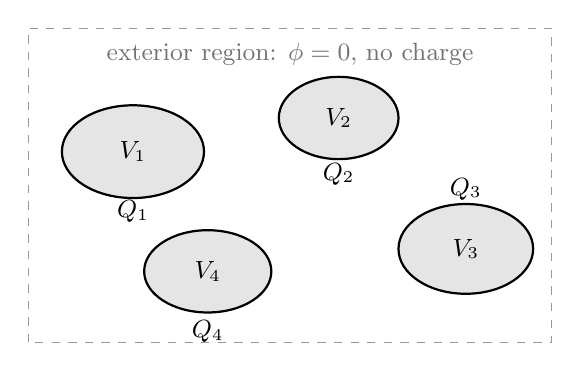
\begin{tikzpicture}[scale=0.95]
  \draw[dashed, black!40] (-3.5,-2.0) rectangle (3.5,2.2);
  \node[font=\small, black!55] at (0,1.85) {exterior region: $\laplacian\phi = 0$, no charge};
  \draw[fill=gray!20, thick] (-2.1,0.55) ellipse (0.95cm and 0.62cm);
  \node[font=\small] at (-2.1,0.55) {$V_1$};
  \draw[fill=gray!20, thick] (0.65,1.0) ellipse (0.8cm and 0.55cm);
  \node[font=\small] at (0.65,1.0) {$V_2$};
  \draw[fill=gray!20, thick] (2.35,-0.75) ellipse (0.9cm and 0.6cm);
  \node[font=\small] at (2.35,-0.75) {$V_3$};
  \draw[fill=gray!20, thick] (-1.1,-1.05) ellipse (0.85cm and 0.55cm);
  \node[font=\small] at (-1.1,-1.05) {$V_4$};
  \node[font=\small] at (-2.1,-0.25) {$Q_1$};
  \node[font=\small] at (0.65,0.25) {$Q_2$};
  \node[font=\small] at (2.35,0.05) {$Q_3$};
  \node[font=\small] at (-1.1,-1.85) {$Q_4$};
\end{tikzpicture}
\end{center}
\caption{A system of $n$ conductors held at prescribed potentials $V_1,\dots,V_n$. The exterior region is charge-free, so $\phi$ is harmonic there, and the potentials on the conductor surfaces are exactly the boundary data that uniqueness says determines it. The charges $Q_i$ are then not free to be chosen --- they are whatever the resulting field puts on each surface.}
\label{fig:em-nconductors}
\end{figure}

\subsection{Elementary Solutions and Superposition}

For each $k = 1,\dots,n$, define the \emph{elementary solution} $\phi^{(k)}(\vect{x})$ to be the potential in the exterior region when conductor $k$ is held at potential $1$ and every other conductor is grounded at potential $0$. Each $\phi^{(k)}$ is harmonic in the exterior region and depends only on the geometry of the conductors --- never on any applied voltage.

\begin{figure}[H]
\begin{center}
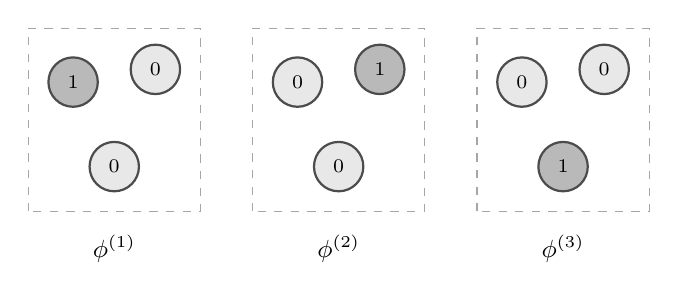
\begin{tikzpicture}[scale=0.95]
\begin{scope}[xshift=0.0cm]
  \draw[dashed, black!35] (-0.15,-0.95) rectangle (2.15,1.5);
  \filldraw[fill=gray!55, draw=black!70, thick] (0.45,0.78) circle (0.33);
  \node[font=\scriptsize] at (0.45,0.78) {$1$};
  \filldraw[fill=gray!18, draw=black!70, thick] (1.55,0.95) circle (0.33);
  \node[font=\scriptsize] at (1.55,0.95) {$0$};
  \filldraw[fill=gray!18, draw=black!70, thick] (1.0,-0.35) circle (0.33);
  \node[font=\scriptsize] at (1.0,-0.35) {$0$};
\end{scope}
\begin{scope}[xshift=3.0cm]
  \draw[dashed, black!35] (-0.15,-0.95) rectangle (2.15,1.5);
  \filldraw[fill=gray!18, draw=black!70, thick] (0.45,0.78) circle (0.33);
  \node[font=\scriptsize] at (0.45,0.78) {$0$};
  \filldraw[fill=gray!55, draw=black!70, thick] (1.55,0.95) circle (0.33);
  \node[font=\scriptsize] at (1.55,0.95) {$1$};
  \filldraw[fill=gray!18, draw=black!70, thick] (1.0,-0.35) circle (0.33);
  \node[font=\scriptsize] at (1.0,-0.35) {$0$};
\end{scope}
\begin{scope}[xshift=6.0cm]
  \draw[dashed, black!35] (-0.15,-0.95) rectangle (2.15,1.5);
  \filldraw[fill=gray!18, draw=black!70, thick] (0.45,0.78) circle (0.33);
  \node[font=\scriptsize] at (0.45,0.78) {$0$};
  \filldraw[fill=gray!18, draw=black!70, thick] (1.55,0.95) circle (0.33);
  \node[font=\scriptsize] at (1.55,0.95) {$0$};
  \filldraw[fill=gray!55, draw=black!70, thick] (1.0,-0.35) circle (0.33);
  \node[font=\scriptsize] at (1.0,-0.35) {$1$};
\end{scope}
\node[font=\small] at (1.0,-1.45) {$\phi^{(1)}$};
\node[font=\small] at (4.0,-1.45) {$\phi^{(2)}$};
\node[font=\small] at (7.0,-1.45) {$\phi^{(3)}$};
\end{tikzpicture}
\end{center}
\caption{The three elementary solutions for a system of $n=3$ conductors. In $\phi^{(k)}$ conductor $k$ is held at potential $1$ (shaded) and every other conductor is grounded at $0$. Each is a complete solution of Laplace's equation in the exterior region, and each depends only on the geometry --- the same three pictures serve for every choice of applied voltages.}
\label{fig:em-elementary}
\end{figure}

\begin{theorem}[Superposition of elementary solutions]
For arbitrary potentials $V_1,\dots,V_n$ on the $n$ conductors, the potential in the exterior region is
\[
    \phi_\text{total}(\vect{x}) = \sum_{k=1}^n V_k\,\phi^{(k)}(\vect{x}).
\]
\end{theorem}

\begin{proof}
Two things must be checked.

\emph{(i) It solves Laplace's equation.} Each $\phi^{(k)}$ is harmonic and $\laplacian$ is linear, so
\[
    \laplacian\phi_\text{total} = \sum_k V_k\,\laplacian\phi^{(k)} = 0 .
\]

\emph{(ii) It matches the prescribed boundary data.} On the surface $S_i$ of conductor $i$, each elementary solution satisfies $\phi^{(k)}\big|_{S_i} = \delta_{ik}$ by construction. Hence
\[
    \phi_\text{total}\Big|_{S_i} = \sum_k V_k\,\phi^{(k)}\Big|_{S_i} = V_i\cdot 1 + \sum_{k\neq i} V_k\cdot 0 = V_i .
\]

Being harmonic in the exterior region and matching the prescribed potential on every conductor's surface, $\phi_\text{total}$ is by uniqueness \emph{the} solution; no other candidate is consistent with this boundary data.
\end{proof}

\begin{figure}[H]
\begin{center}
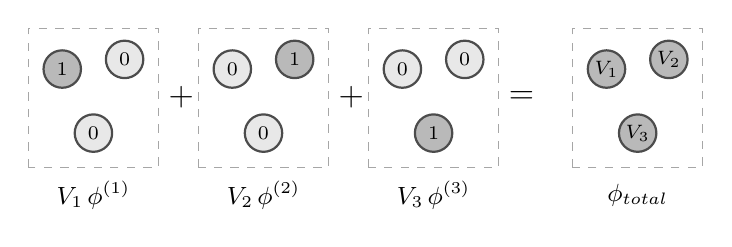
\begin{tikzpicture}[scale=0.72]
\begin{scope}[xshift=0.0cm]
  \draw[dashed, black!35] (-0.15,-0.95) rectangle (2.15,1.5);
  \filldraw[fill=gray!55, draw=black!70, thick] (0.45,0.78) circle (0.33);
  \node[font=\scriptsize] at (0.45,0.78) {$1$};
  \filldraw[fill=gray!18, draw=black!70, thick] (1.55,0.95) circle (0.33);
  \node[font=\scriptsize] at (1.55,0.95) {$0$};
  \filldraw[fill=gray!18, draw=black!70, thick] (1.0,-0.35) circle (0.33);
  \node[font=\scriptsize] at (1.0,-0.35) {$0$};
\end{scope}
\begin{scope}[xshift=3.0cm]
  \draw[dashed, black!35] (-0.15,-0.95) rectangle (2.15,1.5);
  \filldraw[fill=gray!18, draw=black!70, thick] (0.45,0.78) circle (0.33);
  \node[font=\scriptsize] at (0.45,0.78) {$0$};
  \filldraw[fill=gray!55, draw=black!70, thick] (1.55,0.95) circle (0.33);
  \node[font=\scriptsize] at (1.55,0.95) {$1$};
  \filldraw[fill=gray!18, draw=black!70, thick] (1.0,-0.35) circle (0.33);
  \node[font=\scriptsize] at (1.0,-0.35) {$0$};
\end{scope}
\begin{scope}[xshift=6.0cm]
  \draw[dashed, black!35] (-0.15,-0.95) rectangle (2.15,1.5);
  \filldraw[fill=gray!18, draw=black!70, thick] (0.45,0.78) circle (0.33);
  \node[font=\scriptsize] at (0.45,0.78) {$0$};
  \filldraw[fill=gray!18, draw=black!70, thick] (1.55,0.95) circle (0.33);
  \node[font=\scriptsize] at (1.55,0.95) {$0$};
  \filldraw[fill=gray!55, draw=black!70, thick] (1.0,-0.35) circle (0.33);
  \node[font=\scriptsize] at (1.0,-0.35) {$1$};
\end{scope}
\begin{scope}[xshift=9.6cm]
  \draw[dashed, black!35] (-0.15,-0.95) rectangle (2.15,1.5);
  \filldraw[fill=gray!55, draw=black!70, thick] (0.45,0.78) circle (0.33);
  \node[font=\scriptsize] at (0.45,0.78) {$V_1$};
  \filldraw[fill=gray!55, draw=black!70, thick] (1.55,0.95) circle (0.33);
  \node[font=\scriptsize] at (1.55,0.95) {$V_2$};
  \filldraw[fill=gray!55, draw=black!70, thick] (1.0,-0.35) circle (0.33);
  \node[font=\scriptsize] at (1.0,-0.35) {$V_3$};
\end{scope}
\node[font=\large] at (2.55,0.28) {$+$};
\node[font=\large] at (5.55,0.28) {$+$};
\node[font=\large] at (8.55,0.28) {$=$};
\node[font=\small] at (1.0,-1.45) {$V_1\,\phi^{(1)}$};
\node[font=\small] at (4.0,-1.45) {$V_2\,\phi^{(2)}$};
\node[font=\small] at (7.0,-1.45) {$V_3\,\phi^{(3)}$};
\node[font=\small] at (10.6,-1.45) {$\phi_{\text{total}}$};
\end{tikzpicture}
\end{center}
\caption{Superposition. Weighting each elementary solution by the corresponding applied potential and adding gives a function that is harmonic (a sum of harmonic functions) and that takes the value $V_i$ on conductor $i$ (since only the $i$th term is nonzero there). By uniqueness it is therefore \emph{the} solution.}
\label{fig:em-superposition}
\end{figure}

\subsection{The Capacitance Matrix}

The surface charge density on a conductor is $\sigma = -\varepsilon_0\,\pdv*{\phi}{n}$, so the total charge on conductor $i$ is
\[
    Q_i = \oint_{S_i}\sigma\,da = -\varepsilon_0\int_{S_i}\pdv{\phi_\text{total}}{n}\,da .
\]
Substituting the superposition result and using linearity of the integral,
\[
    Q_i = -\varepsilon_0\int_{S_i}\sum_k V_k\,\pdv{\phi^{(k)}}{n}\,da
        = \sum_k V_k\underbrace{\left(-\varepsilon_0\int_{S_i}\pdv{\phi^{(k)}}{n}\,da\right)}_{\displaystyle \equiv\; C_{ik}} .
\]

\begin{formula}[Capacitance matrix]
\[
    Q_i = \sum_{k=1}^n C_{ik}\,V_k .
\]
Each coefficient $C_{ik}$ depends only on the geometry of the conductor system, never on the applied voltages, since it was defined from a problem in which $V_k$ was fixed at exactly $1$ and all other conductors grounded.
\end{formula}

This is the direct $n$-conductor generalization of $Q = C\phi$, and it makes precise the earlier observation that on a system of conductors the charges and potentials are not independent: fixing all the potentials fixes every charge, and the relation between them is linear.

\emph{A check by scaling.} If every $V_j$ is scaled by a common factor $\alpha$, then $\phi\to\alpha\phi$ everywhere by the same linearity-and-uniqueness argument applied directly, and so every $Q_i\to\alpha Q_i$. This is consistent with the formula, since $\sum_k C_{ik}(\alpha V_k) = \alpha\sum_k C_{ik}V_k$.

\begin{figure}[H]
\begin{center}
\begin{tikzpicture}[scale=0.95]
  \draw[fill=gray!35, thick] (-2.3,0) ellipse (1.05cm and 0.78cm);
  \node[font=\small] at (-2.3,0) {$V_k=1$};
  \foreach \a in {20,55,-20,-55} {\node[blue!70!black, font=\scriptsize] at ($(-2.3,0)+(\a:1.15 and 0.9)$) {$+$};}
  \draw[fill=gray!18, thick] (2.3,0) ellipse (1.05cm and 0.78cm);
  \node[font=\small] at (2.3,0) {$V_i=0$};
  \foreach \a in {160,125,200,235} {\node[red, font=\scriptsize] at ($(2.3,0)+(\a:1.15 and 0.9)$) {$-$};}
  \foreach \s in {0.62,0,-0.62} {
    \draw[-{Stealth[length=5pt]}, thick, orange!80!black]
      (-1.2,\s*0.72) to[out=\s*22,in=180-\s*22] (1.2,\s*0.72);
  }
  \node[font=\small] at (0,-1.5) {$C_{ik} = Q_i \le 0$ for $i\neq k$};
  \draw[thick] (2.3,-0.8) -- (2.3,-1.9);
  \foreach \w/\y in {0.42/-1.9, 0.28/-2.05, 0.14/-2.2} {
    \draw[thick] (2.3-\w,\y) -- (2.3+\w,\y);
  }
\end{tikzpicture}
\end{center}
\caption{Why the off-diagonal coefficients are expected to be negative. With conductor $k$ raised to potential $1$ and conductor $i$ grounded, field lines run from the higher potential to the lower and terminate on $i$, depositing charge of the opposite sign. The induced $Q_i$, which is precisely $C_{ik}$, is therefore negative.}
\label{fig:em-offdiagonal}
\end{figure}

\emph{On the off-diagonal entries.} The coefficient $C_{ik}$ with $i\neq k$ is the charge induced on conductor $i$ when conductor $k$ alone is raised to potential $1$ and all others are grounded. Field lines leaving the positively charged conductor $k$ terminate on whichever grounded conductors they reach, including $i$, and by the field-line argument above an induced charge of the opposite sign is expected wherever they terminate. This suggests $C_{ik}\le 0$ for $i\neq k$, in contrast with $C_{ii}>0$. A full proof of that sign pattern, together with the symmetry $C_{ik} = C_{ki}$ --- a consequence of Green's reciprocation theorem --- is a natural next topic.

% =====================================================================
\section{Energy Stored in a Capacitor}
% =====================================================================

\[
  W = \frac{1}{C}\int_0^{Q_f} Q\,dQ = \frac{Q_f^2}{2C} \;\defeq\; U_C
  \qquad \text{-- Energy stored in a Capacitor}
\]

The energy can be written three equivalent ways:

\begin{formula}[Energy stored in a capacitor]
\[
  U_C = \frac{Q^2}{2C} = \frac{Q\Phi}{2} = \frac{1}{2}C\Phi^2
\]
\end{formula}

\noindent For a parallel-plate capacitor with area $A$ and separation $s$:

\[
  C = \frac{\varepsilon_0 A}{s}
  \implies
  U_C = \frac{1}{2}\!\left(\frac{\varepsilon_0 A}{s}\right)\!(E\,s)^2
       = \frac{\varepsilon_0 E^2}{2}\cdot \text{Volume}
\]
where $E = \Phi/s$.

\medskip
\noindent This equation also applies to an \emph{isolated charged conductor}. For an isolated sphere:
\[
  C = 4\pi\varepsilon_0 a, \qquad
  U_C = \frac{1}{2}Cq^2 \;=\; \frac{1}{2}(4\pi\varepsilon_0 a)\Phi^2
      = \frac{1}{2}\cdot\frac{q^2}{4\pi\varepsilon_0 a}
\]
which agrees with the earlier calculation for energy stored in the electric field of a charged sphere.

%%─────────────────────────────────────────────
\subsection{Force Required to Keep Capacitor Plates Apart}
%%─────────────────────────────────────────────

For a general capacitor whose capacitance $C(x)$ depends on plate separation $x$, the plates attract each other and an external force $F_\text{ext}$ is needed to hold them apart. Increasing $x$ by $\Delta x$ at constant $Q$ (one plate fixed) requires the external agent to do work equal to the change in stored energy:

\begin{align*}
  F_\text{ext}\,\Delta x &= \Delta U = \frac{Q^2}{2}\,\frac{\partial}{\partial x}\!\left(\frac{1}{C}\right)\Delta x \\[4pt]
  \implies\quad F_\text{ext} &= \frac{Q^2}{2}\,\frac{d}{dx}\!\left(\frac{1}{C}\right)
\end{align*}


%%─────────────────────────────────────────────
\subsection{Energy Stored per Unit Length (Coaxial Capacitor)}
%%─────────────────────────────────────────────

For the coaxial capacitor above, with $Q = \lambda L$ and $C/L = 2\pi\varepsilon_0/\ln(b/a)$,
\[
  \frac{U}{L} = \frac{1}{L}\cdot\frac{Q^2}{2C} = \frac{\lambda^2}{2}\cdot\frac{L}{C} = \frac{\lambda^2\ln(b/a)}{4\pi\varepsilon_0} .
\]

%%─────────────────────────────────────────────
\subsection{Capacitor Paradox}
%%─────────────────────────────────────────────

The paradox is whether connecting two capacitors in this configuration leaves the field unchanged (A) or causes charge to redistribute so that all field is confined between the inner pair of plates (B). The answer is B: option A contains a logical flaw because $\Delta\phi$ is defined relative to infinity, and assuming nothing changes ignores the fact that the connected plates must equilibrate to a common potential consistent with the boundary conditions at infinity.

\medskip\noindent Note: the end state is one of equilibrium, so every result of this chapter applies to it --- in particular each connected pair is a single conductor, at a single potential throughout.
